% Options for packages loaded elsewhere
\PassOptionsToPackage{unicode}{hyperref}
\PassOptionsToPackage{hyphens}{url}
%
\documentclass[
]{article}
\usepackage{amsmath,amssymb}
\usepackage{lmodern}
\usepackage{iftex}
\ifPDFTeX
  \usepackage[T1]{fontenc}
  \usepackage[utf8]{inputenc}
  \usepackage{textcomp} % provide euro and other symbols
\else % if luatex or xetex
  \usepackage{unicode-math}
  \defaultfontfeatures{Scale=MatchLowercase}
  \defaultfontfeatures[\rmfamily]{Ligatures=TeX,Scale=1}
\fi
% Use upquote if available, for straight quotes in verbatim environments
\IfFileExists{upquote.sty}{\usepackage{upquote}}{}
\IfFileExists{microtype.sty}{% use microtype if available
  \usepackage[]{microtype}
  \UseMicrotypeSet[protrusion]{basicmath} % disable protrusion for tt fonts
}{}
\makeatletter
\@ifundefined{KOMAClassName}{% if non-KOMA class
  \IfFileExists{parskip.sty}{%
    \usepackage{parskip}
  }{% else
    \setlength{\parindent}{0pt}
    \setlength{\parskip}{6pt plus 2pt minus 1pt}}
}{% if KOMA class
  \KOMAoptions{parskip=half}}
\makeatother
\usepackage{xcolor}
\usepackage[margin=1in]{geometry}
\usepackage{color}
\usepackage{fancyvrb}
\newcommand{\VerbBar}{|}
\newcommand{\VERB}{\Verb[commandchars=\\\{\}]}
\DefineVerbatimEnvironment{Highlighting}{Verbatim}{commandchars=\\\{\}}
% Add ',fontsize=\small' for more characters per line
\usepackage{framed}
\definecolor{shadecolor}{RGB}{248,248,248}
\newenvironment{Shaded}{\begin{snugshade}}{\end{snugshade}}
\newcommand{\AlertTok}[1]{\textcolor[rgb]{0.94,0.16,0.16}{#1}}
\newcommand{\AnnotationTok}[1]{\textcolor[rgb]{0.56,0.35,0.01}{\textbf{\textit{#1}}}}
\newcommand{\AttributeTok}[1]{\textcolor[rgb]{0.77,0.63,0.00}{#1}}
\newcommand{\BaseNTok}[1]{\textcolor[rgb]{0.00,0.00,0.81}{#1}}
\newcommand{\BuiltInTok}[1]{#1}
\newcommand{\CharTok}[1]{\textcolor[rgb]{0.31,0.60,0.02}{#1}}
\newcommand{\CommentTok}[1]{\textcolor[rgb]{0.56,0.35,0.01}{\textit{#1}}}
\newcommand{\CommentVarTok}[1]{\textcolor[rgb]{0.56,0.35,0.01}{\textbf{\textit{#1}}}}
\newcommand{\ConstantTok}[1]{\textcolor[rgb]{0.00,0.00,0.00}{#1}}
\newcommand{\ControlFlowTok}[1]{\textcolor[rgb]{0.13,0.29,0.53}{\textbf{#1}}}
\newcommand{\DataTypeTok}[1]{\textcolor[rgb]{0.13,0.29,0.53}{#1}}
\newcommand{\DecValTok}[1]{\textcolor[rgb]{0.00,0.00,0.81}{#1}}
\newcommand{\DocumentationTok}[1]{\textcolor[rgb]{0.56,0.35,0.01}{\textbf{\textit{#1}}}}
\newcommand{\ErrorTok}[1]{\textcolor[rgb]{0.64,0.00,0.00}{\textbf{#1}}}
\newcommand{\ExtensionTok}[1]{#1}
\newcommand{\FloatTok}[1]{\textcolor[rgb]{0.00,0.00,0.81}{#1}}
\newcommand{\FunctionTok}[1]{\textcolor[rgb]{0.00,0.00,0.00}{#1}}
\newcommand{\ImportTok}[1]{#1}
\newcommand{\InformationTok}[1]{\textcolor[rgb]{0.56,0.35,0.01}{\textbf{\textit{#1}}}}
\newcommand{\KeywordTok}[1]{\textcolor[rgb]{0.13,0.29,0.53}{\textbf{#1}}}
\newcommand{\NormalTok}[1]{#1}
\newcommand{\OperatorTok}[1]{\textcolor[rgb]{0.81,0.36,0.00}{\textbf{#1}}}
\newcommand{\OtherTok}[1]{\textcolor[rgb]{0.56,0.35,0.01}{#1}}
\newcommand{\PreprocessorTok}[1]{\textcolor[rgb]{0.56,0.35,0.01}{\textit{#1}}}
\newcommand{\RegionMarkerTok}[1]{#1}
\newcommand{\SpecialCharTok}[1]{\textcolor[rgb]{0.00,0.00,0.00}{#1}}
\newcommand{\SpecialStringTok}[1]{\textcolor[rgb]{0.31,0.60,0.02}{#1}}
\newcommand{\StringTok}[1]{\textcolor[rgb]{0.31,0.60,0.02}{#1}}
\newcommand{\VariableTok}[1]{\textcolor[rgb]{0.00,0.00,0.00}{#1}}
\newcommand{\VerbatimStringTok}[1]{\textcolor[rgb]{0.31,0.60,0.02}{#1}}
\newcommand{\WarningTok}[1]{\textcolor[rgb]{0.56,0.35,0.01}{\textbf{\textit{#1}}}}
\usepackage{graphicx}
\makeatletter
\def\maxwidth{\ifdim\Gin@nat@width>\linewidth\linewidth\else\Gin@nat@width\fi}
\def\maxheight{\ifdim\Gin@nat@height>\textheight\textheight\else\Gin@nat@height\fi}
\makeatother
% Scale images if necessary, so that they will not overflow the page
% margins by default, and it is still possible to overwrite the defaults
% using explicit options in \includegraphics[width, height, ...]{}
\setkeys{Gin}{width=\maxwidth,height=\maxheight,keepaspectratio}
% Set default figure placement to htbp
\makeatletter
\def\fps@figure{htbp}
\makeatother
\setlength{\emergencystretch}{3em} % prevent overfull lines
\providecommand{\tightlist}{%
  \setlength{\itemsep}{0pt}\setlength{\parskip}{0pt}}
\setcounter{secnumdepth}{-\maxdimen} % remove section numbering
\ifLuaTeX
  \usepackage{selnolig}  % disable illegal ligatures
\fi
\IfFileExists{bookmark.sty}{\usepackage{bookmark}}{\usepackage{hyperref}}
\IfFileExists{xurl.sty}{\usepackage{xurl}}{} % add URL line breaks if available
\urlstyle{same} % disable monospaced font for URLs
\hypersetup{
  pdftitle={Homework Assignment \#4},
  pdfauthor={Math 437 - Modern Data Analysis},
  hidelinks,
  pdfcreator={LaTeX via pandoc}}

\title{Homework Assignment \#4}
\author{Math 437 - Modern Data Analysis}
\date{Due Sometime After We Get Back From Spring Break}

\begin{document}
\maketitle

\hypertarget{instructions}{%
\section{Instructions}\label{instructions}}

You should submit either two or three files:

\begin{enumerate}
\def\labelenumi{\arabic{enumi}.}
\tightlist
\item
  You should write your solutions to the Applied Problems and Conceptual
  Problem 3 in this R Markdown file and submit the (.Rmd) file.
\item
  You should knit the final solution file to pdf and submit the pdf. If
  you are having trouble getting code chunks to run, add
  \texttt{eval\ =\ FALSE} to the chunks that do not run. If you are
  having trouble getting R Studio to play nice with your LaTeX
  distribution, I will begrudgingly accept an HTML file instead.
\item
  Solutions to the Key Terms and the other Conceptual Problems can be
  submitted in a separate Word or pdf file or included in the same files
  as your solutions to Conceptual Problem 3 and the Applied Problems.
\end{enumerate}

This homework assignment is worth a total of \textbf{50 points}.

\begin{Shaded}
\begin{Highlighting}[]
\FunctionTok{library}\NormalTok{(ISLR2)}
\FunctionTok{library}\NormalTok{(ggplot2)}
\FunctionTok{library}\NormalTok{(dplyr)}
\FunctionTok{library}\NormalTok{(tidymodels)}
\FunctionTok{library}\NormalTok{(workflows) }
\FunctionTok{library}\NormalTok{(parsnip) }
\FunctionTok{library}\NormalTok{(car)}
\FunctionTok{library}\NormalTok{(discrim)}
\FunctionTok{library}\NormalTok{(klaR)}

\CommentTok{\# You will need other packages to fit models in the Applied Problem}
\CommentTok{\# List them here or as you encounter the need for them}

\NormalTok{misinformation1 }\OtherTok{\textless{}{-}}\NormalTok{ readr}\SpecialCharTok{::}\FunctionTok{read\_csv}\NormalTok{(}\StringTok{"misinformation1.csv"}\NormalTok{)}
\end{Highlighting}
\end{Shaded}

\hypertarget{key-terms-5-pts}{%
\section{Key Terms (5 pts)}\label{key-terms-5-pts}}

Read Chapter 4 of Introduction to Statistical Learning, Second Edition.
Based on your reading, answer the following questions.

\begin{enumerate}
\def\labelenumi{\arabic{enumi}.}
\tightlist
\item
  Explain how to convert probabilities to \emph{odds} and to
  \emph{logits}.
\end{enumerate}

To convert probabilities to odds, we manipulate the logistic function
\(p(X) = e^{\beta_0 + \beta_1X}/(1 + e^{\beta_0 + \beta_1X})\) to solve
for \(e^{\beta_0 + \beta_1X}\). To obtain logits, we take the logarithm
of the manipulated equation to obtain \(log(\frac{p(X)}{1 - p(X)})\).

\begin{enumerate}
\def\labelenumi{\arabic{enumi}.}
\setcounter{enumi}{1}
\tightlist
\item
  Write a sentence to interpret each Coefficient in Table 4.3.
\end{enumerate}

Holding all other predictors constant, for every \(\$1\) increase in
balance, we expect the log odds of default to increase by 0.0057\%.
Holding all other predictors constant, for every \(\$1,000\) increase in
income, we expect the log odds of default to increase by 0.003\%.
Holding all other predictors constant, when compared to non-students, we
expect the log odds of default to decrease by 0.468\% for students.

\begin{enumerate}
\def\labelenumi{\arabic{enumi}.}
\setcounter{enumi}{2}
\tightlist
\item
  Why is the choice of a \emph{baseline} (or \emph{reference level}) for
  the response variable critical when interpreting slopes in multinomial
  logistic regression, but not so much in (standard) logistic
  regression?
\end{enumerate}

In multinomial regression, the choice of baseline affects how we
interpret the log odds, since for each predictors coefficient, we are
interpreting them relative to the chosen baseline. In standard logistic
regression we only have two classes in our response so when we change
our baseline, only the sign of the coefficients change rather than the
value and our interpretation remains the same except for the direction
of change.

\begin{enumerate}
\def\labelenumi{\arabic{enumi}.}
\setcounter{enumi}{3}
\tightlist
\item
  In \emph{Bayes' Theorem} (Equation 4.15), what does \(\pi_k\)
  represent about class \(k\)? What does \(f_k(x)\) represent?
\end{enumerate}

\(\pi_k\) represents the prior probability that a randomly chosen
observation comes from class k. \(f_k(x)\) is the density function of X
for an observation that comes from the kth class. In other words, for
qualitative random variables, it is the probability that an observation
\(X \approx x\) given that the observation comes from the kth class; for
quantitative random variables it is the probability that \(X\) falls
into a small region \(dx\) around \(x\).

\begin{enumerate}
\def\labelenumi{\arabic{enumi}.}
\setcounter{enumi}{4}
\tightlist
\item
  Compare and contrast the assumptions about the predictor(s) in
  \emph{linear discriminant analysis} vs.~\emph{quadratic discriminant
  analysis}. Which approach leads to more complex/flexible models?
\end{enumerate}

In linear discriminant analysis (LDA) we are assuming that within each
class, our observations come from multivariate normal distributions and
that there's a common variance and covariance across classes. In
quadratic discriminant analysis (QDA), we are making the same
assumptions about normality, but we are not assuming that there's a
common covariance matrix across classes. Quadratic discriminant analysis
leads to more complex/flexible models since it is estimating a separate
covariance matrix for each class.

\begin{enumerate}
\def\labelenumi{\arabic{enumi}.}
\setcounter{enumi}{5}
\tightlist
\item
  Use the \emph{confusion matrix} in Table 4.5 to find the
  \emph{sensitivity}, \emph{specificity}, \emph{positive predictive
  value} and \emph{negative predictive value} for this algorithm. It's
  okay to keep your answers as fractions.
\end{enumerate}

Sensitivity = 195/333 Specificity = 9432/9667 positive predictive value
= 195/430 negative predictive value = 9432/9570

\begin{enumerate}
\def\labelenumi{\arabic{enumi}.}
\setcounter{enumi}{6}
\tightlist
\item
  What do the x-axis and y-axis on a \emph{receiver operating
  characteristic} (ROC) curve represent? What is the curve actually a
  function of?
\end{enumerate}

The x-axis represents the false positive rate, and the y-axis represents
the true positive rate. The curve is a function of our threshold value
and how it affects sensitivity and the false positive rate.

\begin{enumerate}
\def\labelenumi{\arabic{enumi}.}
\setcounter{enumi}{7}
\tightlist
\item
  Compare and contrast the assumptions about the predictors in
  \emph{linear discriminant analysis} vs.~\emph{Naive Bayes}. When are
  they equivalent?
\end{enumerate}

In Naive Bayes, we assume the predictors are independent. They are
equivalent when in Naive Bayes, we assume our observations for each
predictor come from normal/Gaussian distributions similar to LDA.

\begin{enumerate}
\def\labelenumi{\arabic{enumi}.}
\setcounter{enumi}{8}
\tightlist
\item
  Consider the five methods compared in Section 4.5.2: LDA, QDA, Naive
  Bayes, Logistic Regression, K-Nearest Neighbors. Which methods would
  you guess to perform best when you suspect the decision boundary to be
  (a) linear, (b) moderately nonlinear, (c) highly complex?
\end{enumerate}

\begin{enumerate}
\def\labelenumi{(\alph{enumi})}
\item
  LDA and logistic regression would likely perform best for linear
  decision boundaries with logisitic regression outperforming LDA when
  assumptions of normality are not met.
\item
  Naive Bayes and QDA would perform best for moderately non-linear
  decision boundaries with Naive Bayes outperforming QDA when there are
  only a small number of observations.
\item
  K-Nearest Neighbors would perform best for highly complex decision
  boundaries given that the appropriate value for K is chosen.
\end{enumerate}

\begin{enumerate}
\def\labelenumi{\arabic{enumi}.}
\setcounter{enumi}{9}
\tightlist
\item
  How does ``regression'' work in a \emph{generalized linear model}?
\end{enumerate}

Regression works by modeling the response, which is assumed to come from
a distribution from the exponential family, and then transforming the
expected value of the response so that this transformed mean is a linear
function of predictors.

\hypertarget{conceptual-problems}{%
\section{Conceptual Problems}\label{conceptual-problems}}

\hypertarget{conceptual-problem-1-2-pts}{%
\subsection{Conceptual Problem 1 (2
pts)}\label{conceptual-problem-1-2-pts}}

Textbook Exercise 4.8.1.

\hypertarget{conceptual-problem-2-4-pts}{%
\subsection{Conceptual Problem 2 (4
pts)}\label{conceptual-problem-2-4-pts}}

\hypertarget{part-a-1-pt}{%
\subsubsection{Part a (1 pt)}\label{part-a-1-pt}}

Textbook Exercise 4.8.2.

\hypertarget{part-b-3-pts}{%
\subsubsection{Part b (3 pts)}\label{part-b-3-pts}}

Suppose that within Group 1, \(X \sim Pois(\lambda_1)\) and within Group
2, \(X \sim Pois(\lambda_2)\). Using techniques employed in the proof in
part (a), find the estimated Bayes decision boundary for classifying an
observation to Group 1 vs.~Group 2. You may assume \(\hat{\lambda_k}\)
is computed as the sample mean of the observations in group \(k\) in the
training set and that \(\hat{\pi}_k\) is computed as the proportion of
observations in the training set that are in group \(k\).

\hypertarget{conceptual-problem-3-6-pts-total}{%
\subsection{Conceptual Problem 3 (6 pts
total)}\label{conceptual-problem-3-6-pts-total}}

Linear discriminant analysis is actually not a Bayesian concept! It was
introduced by Fisher in his analysis of iris data as a dimensionality
reduction method! In this problem, you will follow Fisher's logic and
replicate his discrimination function.

Fisher's original LDA example concerned only the setosa and versicolor
flowers, so we filter the iris dataset to include only those species.

\begin{Shaded}
\begin{Highlighting}[]
\NormalTok{iris\_sv }\OtherTok{\textless{}{-}}\NormalTok{ iris }\SpecialCharTok{\%\textgreater{}\%} \FunctionTok{filter}\NormalTok{(Species }\SpecialCharTok{\%in\%} \FunctionTok{c}\NormalTok{(}\StringTok{"setosa"}\NormalTok{, }\StringTok{"versicolor"}\NormalTok{))}
\end{Highlighting}
\end{Shaded}

\hypertarget{part-a-code-1.5-pts}{%
\subsubsection{Part a (Code: 1.5 pts)}\label{part-a-code-1.5-pts}}

Let \(x_1\) be Sepal Length, \(x_2\) be Sepal Width, \(x_3\) be Petal
Length, and \(x_4\) be Petal Width. Fisher wants to find the linear
combination of the four variables
\(X = \lambda_1 x_1 + \lambda_2 x_2 + \lambda_3 x_3 + \lambda_4 x_4\)
that maximizes the overall ``distance'' in sample means between
\emph{versicolor} and \emph{setosa}, accounting for variation and
covariation within each group.

Specifically, he wants to project this four-dimensional predictor space
into a single dimension along which the ratio \(D^2/S\) is maximized,
where \(D\) is the difference in sample means and \(S\) is the total
within-class sum of squares (i.e., \(SSE\) in an ANOVA table) after
transformation.

Fisher starts by computing a ``sum of squares and products'' matrix S in
each group. The S matrices can be found more easily in R by obtaining
the variance-covariance matrix for the numerical predictors (e.g., using
the \texttt{cov} function) and multiplying the entries by (n-1).
Finally, Fisher adds the S matrices for each group to get the overall
within-class variation.

Using R, create the \texttt{S\_setosa}, \texttt{S\_versicolor}, and
\texttt{S\_overall} matrices.

\begin{Shaded}
\begin{Highlighting}[]
\FunctionTok{head}\NormalTok{(iris\_sv)}
\end{Highlighting}
\end{Shaded}

\begin{verbatim}
##   Sepal.Length Sepal.Width Petal.Length Petal.Width Species
## 1          5.1         3.5          1.4         0.2  setosa
## 2          4.9         3.0          1.4         0.2  setosa
## 3          4.7         3.2          1.3         0.2  setosa
## 4          4.6         3.1          1.5         0.2  setosa
## 5          5.0         3.6          1.4         0.2  setosa
## 6          5.4         3.9          1.7         0.4  setosa
\end{verbatim}

\begin{Shaded}
\begin{Highlighting}[]
\NormalTok{S\_setosa }\OtherTok{\textless{}{-}}\NormalTok{  (}\FunctionTok{cov}\NormalTok{(iris\_sv }\SpecialCharTok{\%\textgreater{}\%} 
                         \FunctionTok{filter}\NormalTok{(Species }\SpecialCharTok{==} \StringTok{"setosa"}\NormalTok{) }\SpecialCharTok{\%\textgreater{}\%} 
\NormalTok{                         dplyr}\SpecialCharTok{::}\FunctionTok{select}\NormalTok{(}\SpecialCharTok{{-}}\NormalTok{Species))}\SpecialCharTok{*}\NormalTok{(}\DecValTok{50{-}1}\NormalTok{))}

\NormalTok{S\_versicolor }\OtherTok{\textless{}{-}}\NormalTok{  (}\FunctionTok{cov}\NormalTok{(iris\_sv }\SpecialCharTok{\%\textgreater{}\%} 
                         \FunctionTok{filter}\NormalTok{(Species }\SpecialCharTok{==} \StringTok{"versicolor"}\NormalTok{) }\SpecialCharTok{\%\textgreater{}\%} 
\NormalTok{                         dplyr}\SpecialCharTok{::}\FunctionTok{select}\NormalTok{(}\SpecialCharTok{{-}}\NormalTok{Species))}\SpecialCharTok{*}\NormalTok{(}\DecValTok{50{-}1}\NormalTok{))}

\NormalTok{S\_overall }\OtherTok{\textless{}{-}}\NormalTok{  S\_setosa }\SpecialCharTok{+}\NormalTok{ S\_versicolor}

\FunctionTok{print}\NormalTok{(S\_setosa)}
\end{Highlighting}
\end{Shaded}

\begin{verbatim}
##              Sepal.Length Sepal.Width Petal.Length Petal.Width
## Sepal.Length       6.0882      4.8616       0.8014      0.5062
## Sepal.Width        4.8616      7.0408       0.5732      0.4556
## Petal.Length       0.8014      0.5732       1.4778      0.2974
## Petal.Width        0.5062      0.4556       0.2974      0.5442
\end{verbatim}

\begin{Shaded}
\begin{Highlighting}[]
\FunctionTok{print}\NormalTok{(S\_versicolor) }
\end{Highlighting}
\end{Shaded}

\begin{verbatim}
##              Sepal.Length Sepal.Width Petal.Length Petal.Width
## Sepal.Length      13.0552       4.174        8.962      2.7332
## Sepal.Width        4.1740       4.825        4.050      2.0190
## Petal.Length       8.9620       4.050       10.820      3.5820
## Petal.Width        2.7332       2.019        3.582      1.9162
\end{verbatim}

\begin{Shaded}
\begin{Highlighting}[]
\FunctionTok{print}\NormalTok{(S\_overall)}
\end{Highlighting}
\end{Shaded}

\begin{verbatim}
##              Sepal.Length Sepal.Width Petal.Length Petal.Width
## Sepal.Length      19.1434      9.0356       9.7634      3.2394
## Sepal.Width        9.0356     11.8658       4.6232      2.4746
## Petal.Length       9.7634      4.6232      12.2978      3.8794
## Petal.Width        3.2394      2.4746       3.8794      2.4604
\end{verbatim}

\hypertarget{part-b-code-1-pt-explanation-0.5-pts}{%
\subsubsection{Part b (Code: 1 pt; Explanation: 0.5
pts)}\label{part-b-code-1-pt-explanation-0.5-pts}}

Fisher then solves a system of four linear equations in four unknowns
(\(\lambda_1\), \(\lambda_2\), \(\lambda_3\), \(\lambda_4\)) that
relates \(S\) to the vector of differences in sample means, i.e.,
\(S \lambda = D\) where \(D\) is the vector of differences in sample
means.

The discriminant function is then the inner product of \(\lambda\) and
\(x\). This solution is unique up to a scaling factor. Fisher suggests
to scale \(\lambda\) such that \(\lambda_1 = 1\).

Using R, solve the matrix equation (\texttt{\%*\%} does matrix
multiplication and \texttt{solve} does matrix inversion) and perform
Fisher's suggested scaling, then write out the discriminant function as
a linear function of \(x_1\), \(x_2\), \(x_3\), \(x_4\).

\(x_1\) be Sepal Length, \(x_2\) be Sepal Width, \(x_3\) be Petal
Length, and \(x_4\) be Petal Width.

\begin{Shaded}
\begin{Highlighting}[]
\NormalTok{iris\_s }\OtherTok{\textless{}{-}}\NormalTok{ iris\_sv }\SpecialCharTok{\%\textgreater{}\%} 
  \FunctionTok{filter}\NormalTok{(Species }\SpecialCharTok{==} \StringTok{"setosa"}\NormalTok{)}

\NormalTok{iris\_v }\OtherTok{\textless{}{-}}\NormalTok{ iris\_sv }\SpecialCharTok{\%\textgreater{}\%} 
  \FunctionTok{filter}\NormalTok{(Species }\SpecialCharTok{==} \StringTok{"versicolor"}\NormalTok{)}

\NormalTok{D }\OtherTok{=} \FunctionTok{matrix}\NormalTok{(}\AttributeTok{data =} \FunctionTok{c}\NormalTok{(}\FunctionTok{mean}\NormalTok{(iris\_s}\SpecialCharTok{$}\NormalTok{Sepal.Length) }\SpecialCharTok{{-}} \FunctionTok{mean}\NormalTok{(iris\_v}\SpecialCharTok{$}\NormalTok{Sepal.Length),}
                    \FunctionTok{mean}\NormalTok{(iris\_s}\SpecialCharTok{$}\NormalTok{Sepal.Width) }\SpecialCharTok{{-}} \FunctionTok{mean}\NormalTok{(iris\_v}\SpecialCharTok{$}\NormalTok{Sepal.Width),}
                    \FunctionTok{mean}\NormalTok{(iris\_s}\SpecialCharTok{$}\NormalTok{Petal.Length) }\SpecialCharTok{{-}} \FunctionTok{mean}\NormalTok{(iris\_v}\SpecialCharTok{$}\NormalTok{Petal.Length),}
                    \FunctionTok{mean}\NormalTok{(iris\_s}\SpecialCharTok{$}\NormalTok{Petal.Width) }\SpecialCharTok{{-}} \FunctionTok{mean}\NormalTok{(iris\_v}\SpecialCharTok{$}\NormalTok{Petal.Width)))}

\NormalTok{lambda }\OtherTok{=} \FunctionTok{solve}\NormalTok{(S\_overall, D)}


\CommentTok{\#Use Sepal Length as our reference level}
\NormalTok{fisher\_scaling }\OtherTok{=}\NormalTok{ lambda }\SpecialCharTok{*} \DecValTok{1}\SpecialCharTok{/}\NormalTok{lambda[}\DecValTok{1}\NormalTok{,}\DecValTok{1}\NormalTok{]}
\end{Highlighting}
\end{Shaded}

\$ Discriminant \space Function = x\_1\emph{1 + x\_2 } 5.9038 -
x\_3\emph{7.1299 -x\_4}10.1037 \$

\hypertarget{part-c-code-1-pt}{%
\subsubsection{Part c (Code: 1 pt)}\label{part-c-code-1-pt}}

Add a new variable to the \texttt{iris\_sv} data frame,
\texttt{discrim}, containing the values of the discriminant function for
each flower. Create a dot plot showing the Species (response) vs.~the
discriminant function value (predictor). You may also want to color-code
by Species.

\begin{Shaded}
\begin{Highlighting}[]
\NormalTok{iris\_sv }\OtherTok{\textless{}{-}}\NormalTok{ iris\_sv }\SpecialCharTok{\%\textgreater{}\%} 
  \FunctionTok{mutate}\NormalTok{(}\AttributeTok{discrim =}\NormalTok{ Sepal.Length}\SpecialCharTok{*}\DecValTok{1} \SpecialCharTok{+}\NormalTok{ Sepal.Width }\SpecialCharTok{*} \FloatTok{5.9038} \SpecialCharTok{{-}}\NormalTok{ Petal.Length}\SpecialCharTok{*}\FloatTok{7.1299} \SpecialCharTok{{-}}\NormalTok{Petal.Width}\SpecialCharTok{*}\FloatTok{10.1037}\NormalTok{)}
\end{Highlighting}
\end{Shaded}

\begin{Shaded}
\begin{Highlighting}[]
\NormalTok{iris\_sv }\SpecialCharTok{\%\textgreater{}\%} 
  \FunctionTok{ggplot}\NormalTok{(}\FunctionTok{aes}\NormalTok{(}\AttributeTok{x =}\NormalTok{ discrim, }\AttributeTok{y =}\NormalTok{ Species, }\AttributeTok{color =}\NormalTok{ Species)) }\SpecialCharTok{+}
  \FunctionTok{geom\_point}\NormalTok{() }
\end{Highlighting}
\end{Shaded}

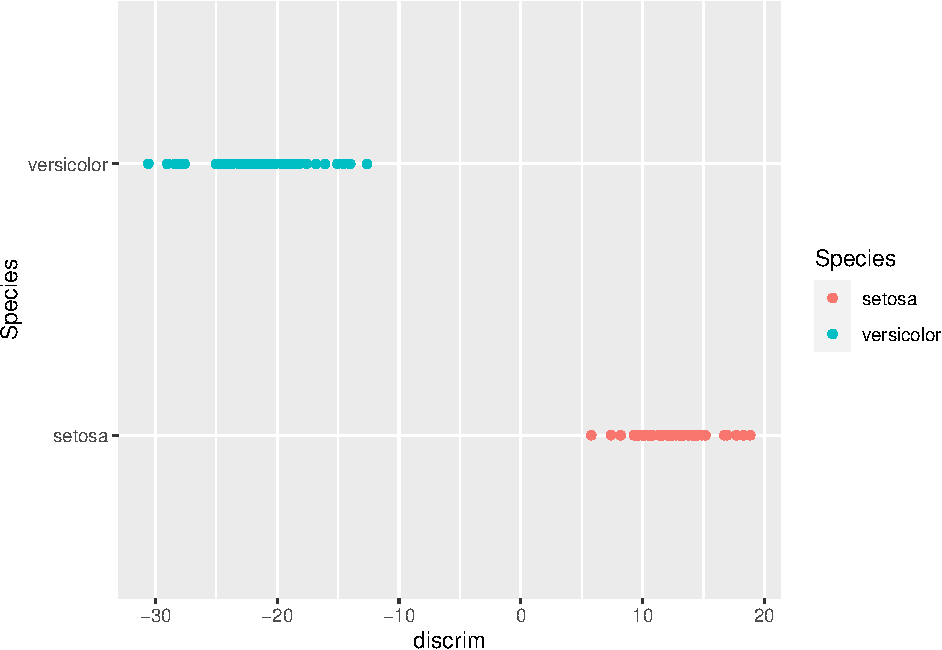
\includegraphics{Homework4_files/figure-latex/unnamed-chunk-4-1.pdf}

\hypertarget{part-d-code-andor-explanation-2-pts}{%
\subsubsection{Part d (Code and/or Explanation: 2
pts)}\label{part-d-code-andor-explanation-2-pts}}

Explain how to use your results to classify a \emph{new} iris flower to
either \emph{setosa} or \emph{versicolor}. (Hint: think about where the
decision boundary is\ldots)

In order to classify a new iris flower we would calculate its'
discriminant and if that value is less than 0 we would predict it to be
veriscolor and if that value were greater than 0 it would be classified
as setosa. (I am assuming that the decision boundary is zero but I am
not 100\% positive)

\hypertarget{applied-problems}{%
\section{Applied Problems}\label{applied-problems}}

\hypertarget{applied-problem-1-33-pts-total}{%
\subsection{Applied Problem 1 (33 pts
total)}\label{applied-problem-1-33-pts-total}}

This problem involves the \texttt{misinformation1} dataset. In 2020,
while biomedical researchers were attempting to develop a vaccine for
COVID-19, public health researchers were attempting to predict whether a
person would get a vaccine once one was available.

The \texttt{misinformation1} dataset contains responses of a subset of
673 Americans to a survey about COVID-19. The \texttt{Vaccine} variable
indicates whether the person said they would get the vaccine (``Yes'')
or said they would not (``No''). Here I create a
\texttt{misinformation2} dataset to convert the \texttt{Vaccine}
variable to a factor variable.

\begin{Shaded}
\begin{Highlighting}[]
\NormalTok{misinformation2 }\OtherTok{\textless{}{-}}\NormalTok{ misinformation1 }\SpecialCharTok{\%\textgreater{}\%} \FunctionTok{mutate}\NormalTok{(}
  \AttributeTok{Vaccine =} \FunctionTok{as.factor}\NormalTok{(Vaccine)}
\NormalTok{)}
\end{Highlighting}
\end{Shaded}

The researchers who analyzed this data believed that people who thought
that COVID-19 was a higher public risk (\texttt{COVID\_Risk}) and people
who had higher trust in scientists (\texttt{Trust\_in\_Scientists})
would be more likely to say they would get the vaccine, while those who
were more susceptible to believing misinformation
(\texttt{Misinformation}) about the vaccine would be less likely to say
they would get the vaccine. So we will use those three predictors in our
models.

\hypertarget{part-a-code-1-pt}{%
\subsubsection{Part a (Code: 1 pt)}\label{part-a-code-1-pt}}

Randomly divide the \texttt{misinformation2} dataset into a holdout set
with 20-25\% of the data (anywhere from 130 to 170 observations is fine)
and a training set with the remaining observations. I used seed
\texttt{222} in my split, but you do not need to replicate my results.
Either the ``Base R'' or the tidymodels (using \texttt{rsample}) way of
doing the split is acceptable.

\begin{Shaded}
\begin{Highlighting}[]
\FunctionTok{set.seed}\NormalTok{(}\DecValTok{222}\NormalTok{)}
\NormalTok{misinfo\_split }\OtherTok{\textless{}{-}} \FunctionTok{initial\_split}\NormalTok{(misinformation2, }\AttributeTok{prop =} \FloatTok{0.75}\NormalTok{)}
\NormalTok{misinfo\_train }\OtherTok{\textless{}{-}} \FunctionTok{training}\NormalTok{(misinfo\_split)}
\NormalTok{misinfo\_test }\OtherTok{\textless{}{-}} \FunctionTok{testing}\NormalTok{(misinfo\_split)}
\end{Highlighting}
\end{Shaded}

\hypertarget{part-b-code-4-pts-explanation-1-pt}{%
\subsubsection{Part b (Code: 4 pts; Explanation: 1
pt)}\label{part-b-code-4-pts-explanation-1-pt}}

Use K-nearest neighbors with a Euclidean distance
(\texttt{dist\_power\ =\ 2}) metric to predict whether someone will get
the COVID-19 vaccine. Use repeated 5-fold cross-validation to find the
optimal value of k, and explain why you chose that value of k. Remember
to do all the necessary preparation work and fit the model on the entire
training set afterwards. It is probably easiest to use a tidymodels
workflow to do this part.

\begin{Shaded}
\begin{Highlighting}[]
\FunctionTok{set.seed}\NormalTok{(}\DecValTok{1002}\NormalTok{)}
\NormalTok{fv\_kfold\_tidy }\OtherTok{\textless{}{-}} \FunctionTok{vfold\_cv}\NormalTok{(misinfo\_train, }\AttributeTok{v =} \DecValTok{5}\NormalTok{, }\AttributeTok{repeats =} \DecValTok{3}\NormalTok{)}
\NormalTok{fv\_kfold\_tidy}
\end{Highlighting}
\end{Shaded}

\begin{verbatim}
## #  5-fold cross-validation repeated 3 times 
## # A tibble: 15 x 3
##    splits            id      id2  
##    <list>            <chr>   <chr>
##  1 <split [403/101]> Repeat1 Fold1
##  2 <split [403/101]> Repeat1 Fold2
##  3 <split [403/101]> Repeat1 Fold3
##  4 <split [403/101]> Repeat1 Fold4
##  5 <split [404/100]> Repeat1 Fold5
##  6 <split [403/101]> Repeat2 Fold1
##  7 <split [403/101]> Repeat2 Fold2
##  8 <split [403/101]> Repeat2 Fold3
##  9 <split [403/101]> Repeat2 Fold4
## 10 <split [404/100]> Repeat2 Fold5
## 11 <split [403/101]> Repeat3 Fold1
## 12 <split [403/101]> Repeat3 Fold2
## 13 <split [403/101]> Repeat3 Fold3
## 14 <split [403/101]> Repeat3 Fold4
## 15 <split [404/100]> Repeat3 Fold5
\end{verbatim}

\begin{Shaded}
\begin{Highlighting}[]
\NormalTok{knn\_model }\OtherTok{\textless{}{-}} \FunctionTok{nearest\_neighbor}\NormalTok{(}\AttributeTok{mode =} \StringTok{"classification"}\NormalTok{, }\AttributeTok{neighbors =} \FunctionTok{tune}\NormalTok{(), }\AttributeTok{dist\_power =} \DecValTok{2}\NormalTok{)}

\NormalTok{knn\_wflow }\OtherTok{\textless{}{-}} \FunctionTok{workflow}\NormalTok{() }\SpecialCharTok{\%\textgreater{}\%}
  \FunctionTok{add\_model}\NormalTok{(knn\_model)}
\end{Highlighting}
\end{Shaded}

\begin{Shaded}
\begin{Highlighting}[]
\NormalTok{knn\_param\_grid }\OtherTok{\textless{}{-}} \FunctionTok{expand.grid}\NormalTok{(}\AttributeTok{neighbors =} \FunctionTok{seq}\NormalTok{(}\DecValTok{1}\NormalTok{, }\DecValTok{10}\NormalTok{))}
\end{Highlighting}
\end{Shaded}

\begin{Shaded}
\begin{Highlighting}[]
\NormalTok{knn\_recipe }\OtherTok{\textless{}{-}} \FunctionTok{recipe}\NormalTok{(}
\NormalTok{  Vaccine }\SpecialCharTok{\textasciitilde{}}\NormalTok{ COVID\_Risk }\SpecialCharTok{+}\NormalTok{ Trust\_in\_Scientists }\SpecialCharTok{+}\NormalTok{ Misinformation, }\CommentTok{\# response \textasciitilde{} predictors}
  \AttributeTok{data =}\NormalTok{ misinfo\_train}
\NormalTok{) }\SpecialCharTok{\%\textgreater{}\%}
  \FunctionTok{step\_normalize}\NormalTok{(}\FunctionTok{all\_numeric\_predictors}\NormalTok{()) }\CommentTok{\# center and scale numeric predictors}
\end{Highlighting}
\end{Shaded}

\begin{Shaded}
\begin{Highlighting}[]
\NormalTok{knn\_tune }\OtherTok{\textless{}{-}} \FunctionTok{tune\_grid}\NormalTok{(knn\_model, }
\NormalTok{                      knn\_recipe, }
                      \AttributeTok{resamples =}\NormalTok{ fv\_kfold\_tidy, }
                      \AttributeTok{grid =}\NormalTok{ knn\_param\_grid)}
\end{Highlighting}
\end{Shaded}

\begin{Shaded}
\begin{Highlighting}[]
\FunctionTok{autoplot}\NormalTok{(knn\_tune)}
\end{Highlighting}
\end{Shaded}

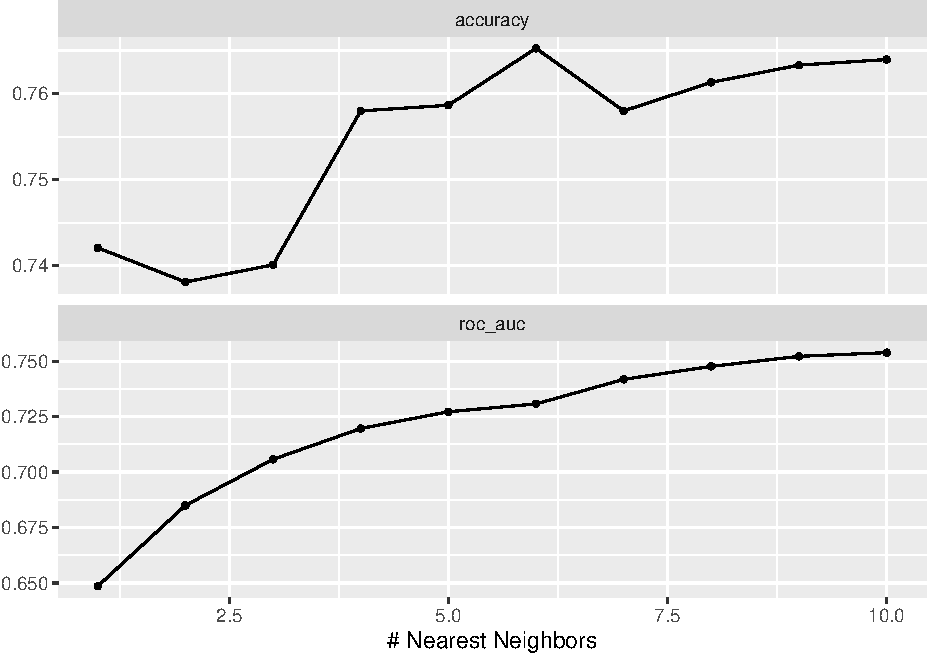
\includegraphics{Homework4_files/figure-latex/unnamed-chunk-7-1.pdf} The
optimal value I chose is k = 6 because it has the highest accuracy.

\hypertarget{part-c-code-1.5-pts-computation-1-pt}{%
\subsubsection{Part c (Code: 1.5 pts; Computation: 1
pt)}\label{part-c-code-1.5-pts-computation-1-pt}}

Make your predictions on the holdout set. Then, obtain the confusion
matrix for this model on the holdout set. Using the confusion matrix,
estimate the accuracy, sensitivity (recall), specificity, positive
predictive value (precision), and negative predictive value for the
K-nearest neighbors model with your optimal value of K.

Confirm your estimates by getting the \texttt{summary} of the confusion
matrix. Remember to use the argument \texttt{event\_level\ =\ "second"}
in the summary function because we want to predict whether someone
\emph{will} get a vaccine.

\begin{Shaded}
\begin{Highlighting}[]
\NormalTok{knn\_model\_final }\OtherTok{\textless{}{-}} \FunctionTok{nearest\_neighbor}\NormalTok{(}\AttributeTok{mode =} \StringTok{"classification"}\NormalTok{, }\AttributeTok{neighbors =} \DecValTok{6}\NormalTok{, }\AttributeTok{dist\_power =} \DecValTok{2}\NormalTok{)}

\NormalTok{knn\_wflow }\OtherTok{\textless{}{-}} \FunctionTok{workflow}\NormalTok{() }\SpecialCharTok{\%\textgreater{}\%}
  \FunctionTok{add\_model}\NormalTok{(knn\_model\_final) }\SpecialCharTok{\%\textgreater{}\%}
  \FunctionTok{add\_recipe}\NormalTok{(knn\_recipe)}


\NormalTok{knn\_fit }\OtherTok{\textless{}{-}} \FunctionTok{fit}\NormalTok{(knn\_wflow, }\AttributeTok{data =}\NormalTok{ misinfo\_train)}

\NormalTok{predictions\_knn\_df }\OtherTok{\textless{}{-}}\NormalTok{ broom}\SpecialCharTok{::}\FunctionTok{augment}\NormalTok{(knn\_fit, }\AttributeTok{new\_data =}\NormalTok{ misinfo\_test)}

\NormalTok{knn\_conf\_mat }\OtherTok{\textless{}{-}} \FunctionTok{conf\_mat}\NormalTok{(predictions\_knn\_df, }\AttributeTok{truth =}\NormalTok{ Vaccine, }\AttributeTok{estimate =}\NormalTok{ .pred\_class)}
\NormalTok{knn\_conf\_mat}
\end{Highlighting}
\end{Shaded}

\begin{verbatim}
##           Truth
## Prediction  No Yes
##        No   27  20
##        Yes  18 104
\end{verbatim}

accuracy: 133/169 = 0.79

sensitivity: TP/TP+FN = 106/124 = 0.85

specificity: TN/TN+FP = 27/45 = 0.6

ppv: TP/TP+FP = 106/124 = 0.85

npv: TN/TN+FN = 27/46 = 0.6

\begin{Shaded}
\begin{Highlighting}[]
\FunctionTok{summary}\NormalTok{(knn\_conf\_mat, }\AttributeTok{event\_level =} \StringTok{"second"}\NormalTok{)}
\end{Highlighting}
\end{Shaded}

\begin{verbatim}
## # A tibble: 13 x 3
##    .metric              .estimator .estimate
##    <chr>                <chr>          <dbl>
##  1 accuracy             binary         0.775
##  2 kap                  binary         0.433
##  3 sens                 binary         0.839
##  4 spec                 binary         0.6  
##  5 ppv                  binary         0.852
##  6 npv                  binary         0.574
##  7 mcc                  binary         0.433
##  8 j_index              binary         0.439
##  9 bal_accuracy         binary         0.719
## 10 detection_prevalence binary         0.722
## 11 precision            binary         0.852
## 12 recall               binary         0.839
## 13 f_meas               binary         0.846
\end{verbatim}

\hypertarget{part-d-code-1-pt-explanation-1-pt}{%
\subsubsection{Part d (Code: 1 pt; Explanation: 1
pt)}\label{part-d-code-1-pt-explanation-1-pt}}

Logistic regression fixes a lot of issues that are present in k-nearest
neighbors. For one thing, we don't have to do any of the pre-processing
and can use the variables on their original scale, which makes
interpretation much easier.

Fit a logistic regression model on the training set predicting
\texttt{Vaccine} from \texttt{COVID\_Risk},
\texttt{Trust\_in\_Scientists}, and \texttt{Misinformation}. Use the
\texttt{glm} function (don't use tidymodels here, because tidymodels
will remove the information you need to do the inference in Part f) with
an appropriate \texttt{family} argument.

Use the \texttt{summary} or \texttt{coef} function to obtain the
coefficient estimates, and write out the equation of the fitted logistic
regression model. You can use either the log-odds formulation or the
probability formulation, but please make sure you are describing what
you are finding the log-odds or probability of.

\begin{Shaded}
\begin{Highlighting}[]
\NormalTok{logr\_misinfo }\OtherTok{\textless{}{-}} \FunctionTok{glm}\NormalTok{(Vaccine }\SpecialCharTok{\textasciitilde{}}\NormalTok{ COVID\_Risk }\SpecialCharTok{+}\NormalTok{ Trust\_in\_Scientists }\SpecialCharTok{+}\NormalTok{ Misinformation, }
                  \AttributeTok{data =}\NormalTok{ misinfo\_train, }\AttributeTok{family =} \StringTok{"binomial"}\NormalTok{)}
\FunctionTok{summary}\NormalTok{(logr\_misinfo)}
\end{Highlighting}
\end{Shaded}

\begin{verbatim}
## 
## Call:
## glm(formula = Vaccine ~ COVID_Risk + Trust_in_Scientists + Misinformation, 
##     family = "binomial", data = misinfo_train)
## 
## Deviance Residuals: 
##     Min       1Q   Median       3Q      Max  
## -2.6574   0.1978   0.4349   0.6856   1.7946  
## 
## Coefficients:
##                     Estimate Std. Error z value Pr(>|z|)    
## (Intercept)         -3.12175    0.71521  -4.365 1.27e-05 ***
## COVID_Risk           0.91610    0.13759   6.658 2.77e-11 ***
## Trust_in_Scientists  0.42697    0.13820   3.089  0.00201 ** 
## Misinformation      -0.39788    0.08936  -4.453 8.49e-06 ***
## ---
## Signif. codes:  0 '***' 0.001 '**' 0.01 '*' 0.05 '.' 0.1 ' ' 1
## 
## (Dispersion parameter for binomial family taken to be 1)
## 
##     Null deviance: 562.40  on 503  degrees of freedom
## Residual deviance: 447.72  on 500  degrees of freedom
## AIC: 455.72
## 
## Number of Fisher Scoring iterations: 5
\end{verbatim}

logit(Someone will get a Vaccine) = -3.12 + 0.92(\texttt{COVID\_Risk}) +
0.43(\texttt{Trust\_in\_Scientists}) - 0.398(\texttt{Misinformation})

\hypertarget{part-e-explanation-2-pts}{%
\subsubsection{Part e (Explanation: 2
pts)}\label{part-e-explanation-2-pts}}

Write a sentence interpreting the coefficient corresponding to
\texttt{Trust\_in\_Scientists} in the logistic regression model. It is
easiest to exponentiate the coefficient and discuss a
\emph{multiplicative} increase in odds.

When \texttt{Trust\_in\_Scientists} increases by one unit, holding all
other predictors in the model constant, the multiplicative increase in
odds of someone saying they will get a vaccine increases by 1.5.

\hypertarget{part-f-code-0.5-pt-explanation-2-pts}{%
\subsubsection{Part f (Code: 0.5 pt; Explanation: 2
pts)}\label{part-f-code-0.5-pt-explanation-2-pts}}

Using the \texttt{confint} function, obtain 95\% confidence intervals
for the parameters of the population logistic regression model. Based on
the confidence intervals, which of the researchers' suspicions about the
relationship between \texttt{Vaccine} and the three predictors can you
conclude are true?

\begin{Shaded}
\begin{Highlighting}[]
\FunctionTok{confint}\NormalTok{(logr\_misinfo, }\AttributeTok{level =} \FloatTok{0.95}\NormalTok{)}
\end{Highlighting}
\end{Shaded}

\begin{verbatim}
## Waiting for profiling to be done...
\end{verbatim}

\begin{verbatim}
##                          2.5 %     97.5 %
## (Intercept)         -4.5603106 -1.7487722
## COVID_Risk           0.6535791  1.1944511
## Trust_in_Scientists  0.1573488  0.7006974
## Misinformation      -0.5741017 -0.2228080
\end{verbatim}

Based on the confidence intervals, we can conclude both of the
scientists suspicions are true. People we thought that COVID-19 was a
higher public risk and people who had higher trust in scientists would
be more likely to say they would get a vaccine. Those who were more
susceptible to believing misinformation about the vaccine would be less
likely to say they would get the vaccine.

\hypertarget{part-g-code-2-pts-computation-1-pt}{%
\subsubsection{Part g (Code: 2 pts; Computation: 1
pt)}\label{part-g-code-2-pts-computation-1-pt}}

Let's make sure we understand how to make class predictions without
using tidymodels.

Use the \texttt{predict} function to obtain predictions for the
validation set. Remember to include the argument
\texttt{type\ =\ "response"} to output predictions as probabilities!
Note that \texttt{augment} is a bit finicky when passing in a
\texttt{glm} object, so you should not use that function here.

Using similar code to Lab 4.7.2 or an \texttt{if\_else} statement,
classify each respondent in the validation set as either getting the
vaccine (``Yes'') or not (``No'') using the estimated Bayes decision
boundary.

Use the \texttt{table} function to obtain the confusion matrix for this
model on the holdout set. Based on the confusion matrix, estimate the
accuracy, sensitivity (recall), specificity, positive predictive value
(precision), and negative predictive value for the logistic regression
model.

Confirm your estimates using the \texttt{conf\_mat} and \texttt{summary}
functions in the \texttt{yardstick} package. Remember to use the
argument \texttt{event\_level\ =\ "second"} in the summary function
because we want to predict whether someone \emph{will} get a vaccine.

\begin{Shaded}
\begin{Highlighting}[]
\NormalTok{predicted\_probs }\OtherTok{\textless{}{-}} \FunctionTok{predict}\NormalTok{(logr\_misinfo, }\AttributeTok{newdata =}\NormalTok{ misinfo\_test, }\AttributeTok{type =} \StringTok{"response"}\NormalTok{)}
\NormalTok{logr\_predictions }\OtherTok{\textless{}{-}} \FunctionTok{tibble}\NormalTok{(}\AttributeTok{Misinformation =}\NormalTok{ misinfo\_test}\SpecialCharTok{$}\NormalTok{Misinformation, }\AttributeTok{Trust\_in\_Scientists =}\NormalTok{ misinfo\_test}\SpecialCharTok{$}\NormalTok{Trust\_in\_Scientists, }\AttributeTok{COVID\_Risk =}\NormalTok{ misinfo\_test}\SpecialCharTok{$}\NormalTok{COVID\_Risk, }\AttributeTok{Vaccine =}\NormalTok{ misinfo\_test}\SpecialCharTok{$}\NormalTok{Vaccine, }\AttributeTok{Prediction =}\NormalTok{ predicted\_probs)}

\NormalTok{p.threshold }\OtherTok{\textless{}{-}} \FloatTok{0.5}

\NormalTok{predicted\_category }\OtherTok{\textless{}{-}} \FunctionTok{if\_else}\NormalTok{(predicted\_probs }\SpecialCharTok{\textgreater{}}\NormalTok{ p.threshold, }\StringTok{"Yes"}\NormalTok{, }\StringTok{"No"}\NormalTok{)}

\NormalTok{logr\_prediction }\OtherTok{\textless{}{-}} \FunctionTok{tibble}\NormalTok{(}\AttributeTok{Misinformation =}\NormalTok{ misinfo\_test}\SpecialCharTok{$}\NormalTok{Misinformation, }\AttributeTok{Trust\_in\_Scientists =}\NormalTok{ misinfo\_test}\SpecialCharTok{$}\NormalTok{Trust\_in\_Scientists, }\AttributeTok{COVID\_Risk =}\NormalTok{ misinfo\_test}\SpecialCharTok{$}\NormalTok{COVID\_Risk, }\AttributeTok{Vaccine =}\NormalTok{ misinfo\_test}\SpecialCharTok{$}\NormalTok{Vaccine, }
                          \AttributeTok{pred\_prob =}\NormalTok{ predicted\_probs, }\AttributeTok{pred\_class =}\NormalTok{ predicted\_category)}

\FunctionTok{table}\NormalTok{(logr\_prediction}\SpecialCharTok{$}\NormalTok{pred\_class, logr\_prediction}\SpecialCharTok{$}\NormalTok{Vaccine, }
      \AttributeTok{dnn =} \FunctionTok{c}\NormalTok{(}\StringTok{"Predicted"}\NormalTok{,}\StringTok{"Actual"}\NormalTok{))}
\end{Highlighting}
\end{Shaded}

\begin{verbatim}
##          Actual
## Predicted  No Yes
##       No   21  10
##       Yes  24 114
\end{verbatim}

accuracy: 135/169 = 0.799

sensitivity: TP/TP+FN = 114/124 = 0.92

specificity: TN/TN+FP = 21/46 = 0.46

ppv: TP/TP+FP = 114/138 = 0.83

npv: TN/TN+FN = 21/31 = 0.68

\begin{Shaded}
\begin{Highlighting}[]
\NormalTok{logr\_prediction}\SpecialCharTok{$}\NormalTok{pred\_class}\OtherTok{\textless{}{-}}\FunctionTok{as.factor}\NormalTok{(logr\_prediction}\SpecialCharTok{$}\NormalTok{pred\_class)}
\NormalTok{logr\_predictions }\OtherTok{\textless{}{-}}\NormalTok{ logr\_predictions }\SpecialCharTok{\%\textgreater{}\%} \FunctionTok{mutate}\NormalTok{(}\AttributeTok{pred\_No =} \DecValTok{1}\SpecialCharTok{{-}}\NormalTok{Prediction)}
\NormalTok{logr\_conf\_mat }\OtherTok{\textless{}{-}} \FunctionTok{conf\_mat}\NormalTok{(logr\_prediction, }\AttributeTok{truth =}\NormalTok{ Vaccine, }\AttributeTok{estimate =}\NormalTok{ pred\_class)}
\NormalTok{logr\_conf\_mat}
\end{Highlighting}
\end{Shaded}

\begin{verbatim}
##           Truth
## Prediction  No Yes
##        No   21  10
##        Yes  24 114
\end{verbatim}

\begin{Shaded}
\begin{Highlighting}[]
\FunctionTok{summary}\NormalTok{(logr\_conf\_mat, }\AttributeTok{event\_level =} \StringTok{"second"}\NormalTok{)}
\end{Highlighting}
\end{Shaded}

\begin{verbatim}
## # A tibble: 13 x 3
##    .metric              .estimator .estimate
##    <chr>                <chr>          <dbl>
##  1 accuracy             binary         0.799
##  2 kap                  binary         0.428
##  3 sens                 binary         0.919
##  4 spec                 binary         0.467
##  5 ppv                  binary         0.826
##  6 npv                  binary         0.677
##  7 mcc                  binary         0.441
##  8 j_index              binary         0.386
##  9 bal_accuracy         binary         0.693
## 10 detection_prevalence binary         0.817
## 11 precision            binary         0.826
## 12 recall               binary         0.919
## 13 f_meas               binary         0.870
\end{verbatim}

\hypertarget{part-h-code-2.5-pts-computation-1-pt}{%
\subsubsection{Part h (Code: 2.5 pts; Computation: 1
pt)}\label{part-h-code-2.5-pts-computation-1-pt}}

Fit a naive Bayes model on the training set predicting \texttt{Vaccine}
from \texttt{COVID\_Risk}, \texttt{Trust\_in\_Scientists}, and
\texttt{Misinformation} and obtain predictions for the holdout set. You
can use either version from lab (using the \texttt{naiveBayes} function
in the e1071 package) or the tidymodels version (using the klaR and
discrim packages).

Obtain the confusion matrix for this model on the holdout set. Using the
confusion matrix, estimate the accuracy, sensitivity (recall),
specificity, positive predictive value (precision), and negative
predictive value for the naive Bayes model.

Confirm your estimates by summarizing the confusion matrix again.
Remember to use the argument \texttt{event\_level\ =\ "second"} in the
summary function because we want to predict whether someone \emph{will}
get a vaccine.

\begin{Shaded}
\begin{Highlighting}[]
\NormalTok{nb\_model }\OtherTok{\textless{}{-}} \FunctionTok{naive\_Bayes}\NormalTok{(}\AttributeTok{mode =} \StringTok{"classification"}\NormalTok{, }\AttributeTok{engine =} \StringTok{"klaR"}\NormalTok{)}

\NormalTok{nb\_wflow }\OtherTok{\textless{}{-}} \FunctionTok{workflow}\NormalTok{() }\SpecialCharTok{\%\textgreater{}\%}
  \FunctionTok{add\_model}\NormalTok{(nb\_model)}
\end{Highlighting}
\end{Shaded}

\begin{Shaded}
\begin{Highlighting}[]
\NormalTok{nb\_recipe }\OtherTok{\textless{}{-}} \FunctionTok{recipe}\NormalTok{(}
\NormalTok{  Vaccine }\SpecialCharTok{\textasciitilde{}}\NormalTok{ Misinformation }\SpecialCharTok{+}\NormalTok{ Trust\_in\_Scientists }\SpecialCharTok{+}\NormalTok{ COVID\_Risk, }
  \AttributeTok{data =}\NormalTok{ misinfo\_train}
\NormalTok{) }\SpecialCharTok{\%\textgreater{}\%} \FunctionTok{step\_dummy}\NormalTok{(}\FunctionTok{all\_nominal\_predictors}\NormalTok{())}

\NormalTok{nb\_wflow }\OtherTok{\textless{}{-}}\NormalTok{ nb\_wflow }\SpecialCharTok{\%\textgreater{}\%}
  \FunctionTok{add\_recipe}\NormalTok{(nb\_recipe)}
\end{Highlighting}
\end{Shaded}

\begin{Shaded}
\begin{Highlighting}[]
\NormalTok{nb\_fit }\OtherTok{\textless{}{-}} \FunctionTok{fit}\NormalTok{(nb\_wflow, }\AttributeTok{data =}\NormalTok{ misinfo\_train)}
\end{Highlighting}
\end{Shaded}

\begin{Shaded}
\begin{Highlighting}[]
\NormalTok{predictions\_nb\_df }\OtherTok{\textless{}{-}}\NormalTok{ broom}\SpecialCharTok{::}\FunctionTok{augment}\NormalTok{(nb\_fit, }\AttributeTok{new\_data =}\NormalTok{ misinfo\_test)}
\NormalTok{predictions\_nb\_df }\SpecialCharTok{\%\textgreater{}\%}\NormalTok{ dplyr}\SpecialCharTok{::}\FunctionTok{select}\NormalTok{(}
\NormalTok{  Vaccine, }
\NormalTok{  .pred\_class, }
\NormalTok{  .pred\_Yes, }
\NormalTok{  .pred\_No)}
\end{Highlighting}
\end{Shaded}

\begin{verbatim}
## # A tibble: 169 x 4
##    Vaccine .pred_class .pred_Yes .pred_No
##    <fct>   <fct>           <dbl>    <dbl>
##  1 Yes     Yes             0.982   0.0176
##  2 Yes     Yes             0.823   0.177 
##  3 Yes     Yes             0.864   0.136 
##  4 Yes     Yes             0.858   0.142 
##  5 No      Yes             0.683   0.317 
##  6 No      No              0.387   0.613 
##  7 No      No              0.217   0.783 
##  8 Yes     Yes             0.873   0.127 
##  9 No      Yes             0.745   0.255 
## 10 No      No              0.395   0.605 
## # ... with 159 more rows
\end{verbatim}

\begin{Shaded}
\begin{Highlighting}[]
\NormalTok{nb\_conf\_mat }\OtherTok{\textless{}{-}} \FunctionTok{conf\_mat}\NormalTok{(predictions\_nb\_df, }\AttributeTok{truth =}\NormalTok{ Vaccine, }\AttributeTok{estimate =}\NormalTok{ .pred\_class)}
\NormalTok{nb\_conf\_mat}
\end{Highlighting}
\end{Shaded}

\begin{verbatim}
##           Truth
## Prediction  No Yes
##        No   27  15
##        Yes  18 109
\end{verbatim}

accuracy: 136/169 = 0.80

sensitivity: TP/TP+FN = 109/124 = 0.88

specificity: TN/TN+FP = 27/45 = 0.6

ppv: TP/TP+FP = 109/127 = 0.86

npv: TN/TN+FN = 27/42 = 0.64

\begin{Shaded}
\begin{Highlighting}[]
\FunctionTok{summary}\NormalTok{(nb\_conf\_mat, }\AttributeTok{event\_level =} \StringTok{"second"}\NormalTok{)}
\end{Highlighting}
\end{Shaded}

\begin{verbatim}
## # A tibble: 13 x 3
##    .metric              .estimator .estimate
##    <chr>                <chr>          <dbl>
##  1 accuracy             binary         0.805
##  2 kap                  binary         0.489
##  3 sens                 binary         0.879
##  4 spec                 binary         0.6  
##  5 ppv                  binary         0.858
##  6 npv                  binary         0.643
##  7 mcc                  binary         0.490
##  8 j_index              binary         0.479
##  9 bal_accuracy         binary         0.740
## 10 detection_prevalence binary         0.751
## 11 precision            binary         0.858
## 12 recall               binary         0.879
## 13 f_meas               binary         0.869
\end{verbatim}

\hypertarget{part-i-code-0.5-pts-explanation-1-pt}{%
\subsubsection{Part i (Code: 0.5 pts; Explanation: 1
pt)}\label{part-i-code-0.5-pts-explanation-1-pt}}

Obtain the correlation matrix and vif for the predictors in the logistic
regression model. Using your results, argue that the major assumption of
naive Bayes is reasonably justified with these predictors.

\begin{Shaded}
\begin{Highlighting}[]
\FunctionTok{vif}\NormalTok{(logr\_misinfo)}
\end{Highlighting}
\end{Shaded}

\begin{verbatim}
##          COVID_Risk Trust_in_Scientists      Misinformation 
##            1.057062            1.080632            1.061278
\end{verbatim}

\begin{Shaded}
\begin{Highlighting}[]
\NormalTok{misinformation2 }\SpecialCharTok{\%\textgreater{}\%} 
\NormalTok{  dplyr}\SpecialCharTok{::}\FunctionTok{select}\NormalTok{(Misinformation, Trust\_in\_Scientists, COVID\_Risk) }\SpecialCharTok{\%\textgreater{}\%} 
  \FunctionTok{cor}\NormalTok{()}
\end{Highlighting}
\end{Shaded}

\begin{verbatim}
##                     Misinformation Trust_in_Scientists COVID_Risk
## Misinformation           1.0000000          -0.3118322 -0.1557215
## Trust_in_Scientists     -0.3118322           1.0000000  0.3706794
## COVID_Risk              -0.1557215           0.3706794  1.0000000
\end{verbatim}

Since our VIF is below 5 and there are not high amounts of correlation
between each group we can reasonably assume
\texttt{Trust\_in\_Scientists}, \texttt{COVID\_Risk}, and
\texttt{Misinformation} are independent.

\hypertarget{part-j-code-2.5-pts-computation-1-pt}{%
\subsubsection{Part j (Code: 2.5 pts; Computation: 1
pt)}\label{part-j-code-2.5-pts-computation-1-pt}}

Fit a linear discriminant analysis (LDA) model on the training set
predicting \texttt{Vaccine} from \texttt{COVID\_Risk},
\texttt{Trust\_in\_Scientists}, and \texttt{Misinformation} and obtain
predictions for the holdout set. You should use the \texttt{lda}
function in the MASS package but can use it either by itself (as shown
in the lab) or as the ``engine'' in the tidymodels workflow.

Obtain the confusion matrix for this model on the holdout set. Using the
confusion matrix, estimate the accuracy, sensitivity (recall),
specificity, positive predictive value (precision), and negative
predictive value for the LDA model.

Confirm your estimates by summarizing the confusion matrix again.
Remember to use the argument \texttt{event\_level\ =\ "second"} in the
summary function because we want to predict whether someone \emph{will}
get a vaccine.

\begin{Shaded}
\begin{Highlighting}[]
\NormalTok{lda\_model }\OtherTok{\textless{}{-}} \FunctionTok{discrim\_linear}\NormalTok{(}\AttributeTok{mode =} \StringTok{"classification"}\NormalTok{, }\AttributeTok{engine =} \StringTok{"MASS"}\NormalTok{)}

\NormalTok{lda\_wflow }\OtherTok{\textless{}{-}} \FunctionTok{workflow}\NormalTok{() }\SpecialCharTok{\%\textgreater{}\%}
  \FunctionTok{add\_model}\NormalTok{(lda\_model)}
\end{Highlighting}
\end{Shaded}

\begin{Shaded}
\begin{Highlighting}[]
\NormalTok{lda\_wflow }\OtherTok{\textless{}{-}}\NormalTok{ lda\_wflow }\SpecialCharTok{\%\textgreater{}\%}
  \FunctionTok{add\_recipe}\NormalTok{(nb\_recipe)}
\end{Highlighting}
\end{Shaded}

\begin{Shaded}
\begin{Highlighting}[]
\NormalTok{lda\_fit }\OtherTok{\textless{}{-}} \FunctionTok{fit}\NormalTok{(lda\_wflow, }\AttributeTok{data =}\NormalTok{ misinfo\_train)}
\end{Highlighting}
\end{Shaded}

\begin{Shaded}
\begin{Highlighting}[]
\NormalTok{predictions\_lda\_df }\OtherTok{\textless{}{-}}\NormalTok{ broom}\SpecialCharTok{::}\FunctionTok{augment}\NormalTok{(lda\_fit, }\AttributeTok{new\_data =}\NormalTok{ misinfo\_test)}
\NormalTok{predictions\_lda\_df }\SpecialCharTok{\%\textgreater{}\%}\NormalTok{ dplyr}\SpecialCharTok{::}\FunctionTok{select}\NormalTok{(}
\NormalTok{  Vaccine, }
\NormalTok{  .pred\_class, }
\NormalTok{  .pred\_Yes, }
\NormalTok{  .pred\_No)}
\end{Highlighting}
\end{Shaded}

\begin{verbatim}
## # A tibble: 169 x 4
##    Vaccine .pred_class .pred_Yes .pred_No
##    <fct>   <fct>           <dbl>    <dbl>
##  1 Yes     Yes             0.961   0.0388
##  2 Yes     Yes             0.843   0.157 
##  3 Yes     Yes             0.886   0.114 
##  4 Yes     Yes             0.757   0.243 
##  5 No      Yes             0.748   0.252 
##  6 No      Yes             0.551   0.449 
##  7 No      No              0.339   0.661 
##  8 Yes     Yes             0.862   0.138 
##  9 No      Yes             0.633   0.367 
## 10 No      Yes             0.569   0.431 
## # ... with 159 more rows
\end{verbatim}

\begin{Shaded}
\begin{Highlighting}[]
\NormalTok{lda\_conf\_mat }\OtherTok{\textless{}{-}} \FunctionTok{conf\_mat}\NormalTok{(predictions\_lda\_df, }\AttributeTok{truth =}\NormalTok{ Vaccine, }\AttributeTok{estimate =}\NormalTok{ .pred\_class)}
\NormalTok{lda\_conf\_mat}
\end{Highlighting}
\end{Shaded}

\begin{verbatim}
##           Truth
## Prediction  No Yes
##        No   21  11
##        Yes  24 113
\end{verbatim}

accuracy: 134/169 = 0.79

sensitivity: TP/TP+FN = 113/124 = 0.91

specificity: TN/TN+FP = 21/45 = 0.47

ppv: TP/TP+FP = 113/137 = 0.82

npv: TN/TN+FN = 21/32 = 0.66

\begin{Shaded}
\begin{Highlighting}[]
\FunctionTok{summary}\NormalTok{(lda\_conf\_mat, }\AttributeTok{event\_level =} \StringTok{"second"}\NormalTok{)}
\end{Highlighting}
\end{Shaded}

\begin{verbatim}
## # A tibble: 13 x 3
##    .metric              .estimator .estimate
##    <chr>                <chr>          <dbl>
##  1 accuracy             binary         0.793
##  2 kap                  binary         0.416
##  3 sens                 binary         0.911
##  4 spec                 binary         0.467
##  5 ppv                  binary         0.825
##  6 npv                  binary         0.656
##  7 mcc                  binary         0.426
##  8 j_index              binary         0.378
##  9 bal_accuracy         binary         0.689
## 10 detection_prevalence binary         0.811
## 11 precision            binary         0.825
## 12 recall               binary         0.911
## 13 f_meas               binary         0.866
\end{verbatim}

\hypertarget{part-k-code-3-pts}{%
\subsubsection{Part k (Code: 3 pts)}\label{part-k-code-3-pts}}

For each of the four models, obtain the Matthews Correlation
Coefficient, (mean) log-loss, and Brier score.

\begin{Shaded}
\begin{Highlighting}[]
\FunctionTok{summary}\NormalTok{(knn\_conf\_mat, }\AttributeTok{event\_level =} \StringTok{"second"}\NormalTok{) }\SpecialCharTok{\%\textgreater{}\%} \FunctionTok{filter}\NormalTok{(.metric }\SpecialCharTok{==} \StringTok{"mcc"}\NormalTok{)}
\end{Highlighting}
\end{Shaded}

\begin{verbatim}
## # A tibble: 1 x 3
##   .metric .estimator .estimate
##   <chr>   <chr>          <dbl>
## 1 mcc     binary         0.433
\end{verbatim}

\begin{Shaded}
\begin{Highlighting}[]
\NormalTok{brier\_knn }\OtherTok{\textless{}{-}}\NormalTok{ predictions\_knn\_df }\SpecialCharTok{\%\textgreater{}\%} \FunctionTok{mutate}\NormalTok{(}
  \AttributeTok{squared\_error =} \FunctionTok{case\_when}\NormalTok{(}
\NormalTok{    .pred\_class }\SpecialCharTok{==} \StringTok{"Yes"} \SpecialCharTok{\textasciitilde{}}\NormalTok{ (}\DecValTok{1} \SpecialCharTok{{-}}\NormalTok{ .pred\_Yes)}\SpecialCharTok{\^{}}\DecValTok{2}\NormalTok{,}
\NormalTok{    .pred\_class }\SpecialCharTok{==} \StringTok{"No"} \SpecialCharTok{\textasciitilde{}}\NormalTok{ (}\DecValTok{1} \SpecialCharTok{{-}}\NormalTok{ .pred\_No)}\SpecialCharTok{\^{}}\DecValTok{2}
\NormalTok{  )}
\NormalTok{)}
\FunctionTok{mean}\NormalTok{(brier\_knn}\SpecialCharTok{$}\NormalTok{squared\_error)}
\end{Highlighting}
\end{Shaded}

\begin{verbatim}
## [1] 0.05466918
\end{verbatim}

\begin{Shaded}
\begin{Highlighting}[]
\FunctionTok{mn\_log\_loss}\NormalTok{(predictions\_knn\_df,}
            \AttributeTok{truth =}\NormalTok{ Vaccine,}
\NormalTok{            .pred\_Yes,}
            \AttributeTok{event\_level =} \StringTok{"second"}
\NormalTok{)}
\end{Highlighting}
\end{Shaded}

\begin{verbatim}
## # A tibble: 1 x 3
##   .metric     .estimator .estimate
##   <chr>       <chr>          <dbl>
## 1 mn_log_loss binary          2.13
\end{verbatim}

\begin{Shaded}
\begin{Highlighting}[]
\FunctionTok{summary}\NormalTok{(logr\_conf\_mat, }\AttributeTok{event\_level =} \StringTok{"second"}\NormalTok{) }\SpecialCharTok{\%\textgreater{}\%} \FunctionTok{filter}\NormalTok{(.metric }\SpecialCharTok{==} \StringTok{"mcc"}\NormalTok{)}
\end{Highlighting}
\end{Shaded}

\begin{verbatim}
## # A tibble: 1 x 3
##   .metric .estimator .estimate
##   <chr>   <chr>          <dbl>
## 1 mcc     binary         0.441
\end{verbatim}

\begin{Shaded}
\begin{Highlighting}[]
\NormalTok{logr\_predictions }\OtherTok{\textless{}{-}}\NormalTok{ logr\_predictions }\SpecialCharTok{\%\textgreater{}\%} \FunctionTok{mutate}\NormalTok{(}\AttributeTok{pred\_Class =}\NormalTok{ predicted\_category)}
\NormalTok{brier\_nb }\OtherTok{\textless{}{-}}\NormalTok{ logr\_predictions }\SpecialCharTok{\%\textgreater{}\%} \FunctionTok{mutate}\NormalTok{(}
  \AttributeTok{squared\_error =} \FunctionTok{case\_when}\NormalTok{(}
\NormalTok{    pred\_Class }\SpecialCharTok{==} \StringTok{"Yes"} \SpecialCharTok{\textasciitilde{}}\NormalTok{ (}\DecValTok{1} \SpecialCharTok{{-}}\NormalTok{ Prediction)}\SpecialCharTok{\^{}}\DecValTok{2}\NormalTok{,}
\NormalTok{    pred\_Class }\SpecialCharTok{==} \StringTok{"No"} \SpecialCharTok{\textasciitilde{}}\NormalTok{ (}\DecValTok{1} \SpecialCharTok{{-}}\NormalTok{ pred\_No)}\SpecialCharTok{\^{}}\DecValTok{2}
\NormalTok{  )}
\NormalTok{)}
\FunctionTok{mean}\NormalTok{(brier\_nb}\SpecialCharTok{$}\NormalTok{squared\_error)}
\end{Highlighting}
\end{Shaded}

\begin{verbatim}
## [1] 0.06186946
\end{verbatim}

\begin{Shaded}
\begin{Highlighting}[]
\FunctionTok{mn\_log\_loss}\NormalTok{(logr\_predictions,}
            \AttributeTok{truth =}\NormalTok{ Vaccine,}
\NormalTok{            Prediction,}
            \AttributeTok{event\_level =} \StringTok{"second"}
\NormalTok{)}
\end{Highlighting}
\end{Shaded}

\begin{verbatim}
## # A tibble: 1 x 3
##   .metric     .estimator .estimate
##   <chr>       <chr>          <dbl>
## 1 mn_log_loss binary         0.472
\end{verbatim}

\begin{Shaded}
\begin{Highlighting}[]
\FunctionTok{summary}\NormalTok{(nb\_conf\_mat, }\AttributeTok{event\_level =} \StringTok{"second"}\NormalTok{) }\SpecialCharTok{\%\textgreater{}\%} \FunctionTok{filter}\NormalTok{(.metric }\SpecialCharTok{==} \StringTok{"mcc"}\NormalTok{)}
\end{Highlighting}
\end{Shaded}

\begin{verbatim}
## # A tibble: 1 x 3
##   .metric .estimator .estimate
##   <chr>   <chr>          <dbl>
## 1 mcc     binary         0.490
\end{verbatim}

\begin{Shaded}
\begin{Highlighting}[]
\NormalTok{brier\_nb }\OtherTok{\textless{}{-}}\NormalTok{ predictions\_nb\_df }\SpecialCharTok{\%\textgreater{}\%} \FunctionTok{mutate}\NormalTok{(}
  \AttributeTok{squared\_error =} \FunctionTok{case\_when}\NormalTok{(}
\NormalTok{    .pred\_class }\SpecialCharTok{==} \StringTok{"Yes"} \SpecialCharTok{\textasciitilde{}}\NormalTok{ (}\DecValTok{1} \SpecialCharTok{{-}}\NormalTok{ .pred\_Yes)}\SpecialCharTok{\^{}}\DecValTok{2}\NormalTok{,}
\NormalTok{    .pred\_class }\SpecialCharTok{==} \StringTok{"No"} \SpecialCharTok{\textasciitilde{}}\NormalTok{ (}\DecValTok{1} \SpecialCharTok{{-}}\NormalTok{ .pred\_No)}\SpecialCharTok{\^{}}\DecValTok{2}
\NormalTok{  )}
\NormalTok{)}
\FunctionTok{mean}\NormalTok{(brier\_nb}\SpecialCharTok{$}\NormalTok{squared\_error)}
\end{Highlighting}
\end{Shaded}

\begin{verbatim}
## [1] 0.04854214
\end{verbatim}

\begin{Shaded}
\begin{Highlighting}[]
\FunctionTok{mn\_log\_loss}\NormalTok{(predictions\_nb\_df,}
            \AttributeTok{truth =}\NormalTok{ Vaccine,}
\NormalTok{            .pred\_Yes,}
            \AttributeTok{event\_level =} \StringTok{"second"}
\NormalTok{)}
\end{Highlighting}
\end{Shaded}

\begin{verbatim}
## # A tibble: 1 x 3
##   .metric     .estimator .estimate
##   <chr>       <chr>          <dbl>
## 1 mn_log_loss binary         0.481
\end{verbatim}

\begin{Shaded}
\begin{Highlighting}[]
\FunctionTok{summary}\NormalTok{(lda\_conf\_mat, }\AttributeTok{event\_level =} \StringTok{"second"}\NormalTok{) }\SpecialCharTok{\%\textgreater{}\%} \FunctionTok{filter}\NormalTok{(.metric }\SpecialCharTok{==} \StringTok{"mcc"}\NormalTok{)}
\end{Highlighting}
\end{Shaded}

\begin{verbatim}
## # A tibble: 1 x 3
##   .metric .estimator .estimate
##   <chr>   <chr>          <dbl>
## 1 mcc     binary         0.426
\end{verbatim}

\begin{Shaded}
\begin{Highlighting}[]
\NormalTok{brier\_lda }\OtherTok{\textless{}{-}}\NormalTok{ predictions\_lda\_df }\SpecialCharTok{\%\textgreater{}\%} \FunctionTok{mutate}\NormalTok{(}
  \AttributeTok{squared\_error =} \FunctionTok{case\_when}\NormalTok{(}
\NormalTok{    .pred\_class }\SpecialCharTok{==} \StringTok{"Yes"} \SpecialCharTok{\textasciitilde{}}\NormalTok{ (}\DecValTok{1} \SpecialCharTok{{-}}\NormalTok{ .pred\_Yes)}\SpecialCharTok{\^{}}\DecValTok{2}\NormalTok{,}
\NormalTok{    .pred\_class }\SpecialCharTok{==} \StringTok{"No"} \SpecialCharTok{\textasciitilde{}}\NormalTok{ (}\DecValTok{1} \SpecialCharTok{{-}}\NormalTok{ .pred\_No)}\SpecialCharTok{\^{}}\DecValTok{2}
\NormalTok{  )}
\NormalTok{)}
\FunctionTok{mean}\NormalTok{(brier\_lda}\SpecialCharTok{$}\NormalTok{squared\_error)}
\end{Highlighting}
\end{Shaded}

\begin{verbatim}
## [1] 0.05847291
\end{verbatim}

\begin{Shaded}
\begin{Highlighting}[]
\FunctionTok{mn\_log\_loss}\NormalTok{(predictions\_lda\_df,}
            \AttributeTok{truth =}\NormalTok{ Vaccine,}
\NormalTok{            .pred\_Yes,}
            \AttributeTok{event\_level =} \StringTok{"second"}
\NormalTok{)}
\end{Highlighting}
\end{Shaded}

\begin{verbatim}
## # A tibble: 1 x 3
##   .metric     .estimator .estimate
##   <chr>       <chr>          <dbl>
## 1 mn_log_loss binary         0.475
\end{verbatim}

\hypertarget{part-l-code-2-pts}{%
\subsubsection{Part l (Code: 2 pts)}\label{part-l-code-2-pts}}

For each of the four models, produce a plot of the receiver operating
characteristic (ROC) curve, and obtain the area under the curve (AUC).

\begin{Shaded}
\begin{Highlighting}[]
\CommentTok{\# Construct the ROC curve}
\NormalTok{roc\_tibble\_knn }\OtherTok{\textless{}{-}} \FunctionTok{roc\_curve}\NormalTok{(predictions\_knn\_df, }\AttributeTok{truth =}\NormalTok{ Vaccine, .pred\_No)}
\end{Highlighting}
\end{Shaded}

\begin{verbatim}
## Warning: Returning more (or less) than 1 row per `summarise()` group was deprecated in
## dplyr 1.1.0.
## i Please use `reframe()` instead.
## i When switching from `summarise()` to `reframe()`, remember that `reframe()`
##   always returns an ungrouped data frame and adjust accordingly.
## i The deprecated feature was likely used in the yardstick package.
##   Please report the issue at <]8;;https://github.com/tidymodels/yardstick/issueshttps://github.com/tidymodels/yardstick/issues]8;;>.
\end{verbatim}

\begin{Shaded}
\begin{Highlighting}[]
\CommentTok{\# Plot the ROC curve}
\FunctionTok{autoplot}\NormalTok{(roc\_tibble\_knn) }\SpecialCharTok{+} \FunctionTok{labs}\NormalTok{(}\AttributeTok{title =} \StringTok{"ROC Curve for Test Set"}\NormalTok{)}
\end{Highlighting}
\end{Shaded}

\includegraphics{Homework4_files/figure-latex/ROC curve - knn-1.pdf}

\begin{Shaded}
\begin{Highlighting}[]
\FunctionTok{roc\_auc}\NormalTok{(predictions\_knn\_df, }\AttributeTok{truth =}\NormalTok{ Vaccine, .pred\_No)}
\end{Highlighting}
\end{Shaded}

\begin{verbatim}
## # A tibble: 1 x 3
##   .metric .estimator .estimate
##   <chr>   <chr>          <dbl>
## 1 roc_auc binary         0.735
\end{verbatim}

\begin{Shaded}
\begin{Highlighting}[]
\CommentTok{\# Construct the ROC curve}
\NormalTok{roc\_tibble\_logr }\OtherTok{\textless{}{-}} \FunctionTok{roc\_curve}\NormalTok{(logr\_predictions, }\AttributeTok{truth =}\NormalTok{ Vaccine, pred\_No)}

\CommentTok{\# Plot the ROC curve}
\FunctionTok{autoplot}\NormalTok{(roc\_tibble\_logr) }\SpecialCharTok{+} \FunctionTok{labs}\NormalTok{(}\AttributeTok{title =} \StringTok{"ROC Curve for Test Set"}\NormalTok{)}
\end{Highlighting}
\end{Shaded}

\includegraphics{Homework4_files/figure-latex/ROC curve - logr-1.pdf}

\begin{Shaded}
\begin{Highlighting}[]
\FunctionTok{roc\_auc}\NormalTok{(logr\_predictions, }\AttributeTok{truth =}\NormalTok{ Vaccine, pred\_No)}
\end{Highlighting}
\end{Shaded}

\begin{verbatim}
## # A tibble: 1 x 3
##   .metric .estimator .estimate
##   <chr>   <chr>          <dbl>
## 1 roc_auc binary         0.787
\end{verbatim}

\begin{Shaded}
\begin{Highlighting}[]
\CommentTok{\# Construct the ROC curve}
\NormalTok{roc\_tibble\_nb }\OtherTok{\textless{}{-}} \FunctionTok{roc\_curve}\NormalTok{(predictions\_nb\_df, }\AttributeTok{truth =}\NormalTok{ Vaccine, .pred\_No)}

\CommentTok{\# Plot the ROC curve}
\FunctionTok{autoplot}\NormalTok{(roc\_tibble\_nb) }\SpecialCharTok{+} \FunctionTok{labs}\NormalTok{(}\AttributeTok{title =} \StringTok{"ROC Curve for Test Set"}\NormalTok{)}
\end{Highlighting}
\end{Shaded}

\includegraphics{Homework4_files/figure-latex/ROC curve - nb-1.pdf}

\begin{Shaded}
\begin{Highlighting}[]
\FunctionTok{roc\_auc}\NormalTok{(predictions\_nb\_df, }\AttributeTok{truth =}\NormalTok{ Vaccine, .pred\_No)}
\end{Highlighting}
\end{Shaded}

\begin{verbatim}
## # A tibble: 1 x 3
##   .metric .estimator .estimate
##   <chr>   <chr>          <dbl>
## 1 roc_auc binary         0.802
\end{verbatim}

\begin{Shaded}
\begin{Highlighting}[]
\CommentTok{\# Construct the ROC curve}
\NormalTok{roc\_tibble\_lda }\OtherTok{\textless{}{-}} \FunctionTok{roc\_curve}\NormalTok{(predictions\_lda\_df, }\AttributeTok{truth =}\NormalTok{ Vaccine, .pred\_No)}

\CommentTok{\# Plot the ROC curve}
\FunctionTok{autoplot}\NormalTok{(roc\_tibble\_lda) }\SpecialCharTok{+} \FunctionTok{labs}\NormalTok{(}\AttributeTok{title =} \StringTok{"ROC Curve for Test Set"}\NormalTok{)}
\end{Highlighting}
\end{Shaded}

\includegraphics{Homework4_files/figure-latex/ROC curve - lda-1.pdf}

\begin{Shaded}
\begin{Highlighting}[]
\FunctionTok{roc\_auc}\NormalTok{(predictions\_lda\_df, }\AttributeTok{truth =}\NormalTok{ Vaccine, .pred\_No)}
\end{Highlighting}
\end{Shaded}

\begin{verbatim}
## # A tibble: 1 x 3
##   .metric .estimator .estimate
##   <chr>   <chr>          <dbl>
## 1 roc_auc binary         0.785
\end{verbatim}

\hypertarget{part-m-explanation-1.5-pts}{%
\subsubsection{Part m (Explanation: 1.5
pts)}\label{part-m-explanation-1.5-pts}}

Which of the four models you fit (k-nn, logistic regression, naive
Bayes, or LDA) would you argue is the ``best'' model for predicting
whether or not someone would get a COVID-19 vaccine? Justify your answer
based on a metric \emph{other} than accuracy.

Based on the Brier score for each model, the naive Bayes model is the
``best'' model. This model has the lowest Brier score compared to the
others at 0.049.

\end{document}
